\section{Data Driven Background Estimation Methods}
\label{sec:datadriven}

For the high \pt\ dilepton trigger sample, we use 3 data-driven methods to 
estimate the background in the signal region. The first one exploits the fact that 
\Ht\ and $y$ are nearly uncorrelated for the $t\bar{t}$ background The second one 
is based on the fact that in $t\bar{t}$ the \pt\ of the dilepton pair is on average 
nearly the same as the \pt\ of the pair of neutrinos
from $W$-decays, which is reconstructed as \met\ in the
detector. The third method exploits the fact that in \ttbar\ events
the rates of same-flavor vs. opposite-flavor dilepton events are
the same. For the low lepton \pt\ events collected by the dilepton-\Ht\ triggers,
we use the opposite-flavor subtraction technique.

We study the closure of these methods using our madgraph \ttbar\ sample, as well as 
the powheg sample \\
TTTo2L2Nu2B\_7TeV-powheg-pythia6\_Spring11-PU\_S1\_START311\_V1G1-v1
which has approximately 10 times more events in the dilepton channel than the madgraph sample.
We use these samples to estimate correction factors and systematic uncertainties for the background predictions. 
However, the final choice of correction factors and uncertainties will be extracted from the Summer11 \ttbar\ madgraph
sample which will have 50 times as many events as the current madgraph sample. 
For the studies presented in this section, we do not apply trigger efficiency corrections or reweighting for
number of reconstructed vertices since are not comparing MC to data. 

\subsection{ABCD method}
\label{sec:abcd}


\begin{figure}[hbt]
\begin{center}
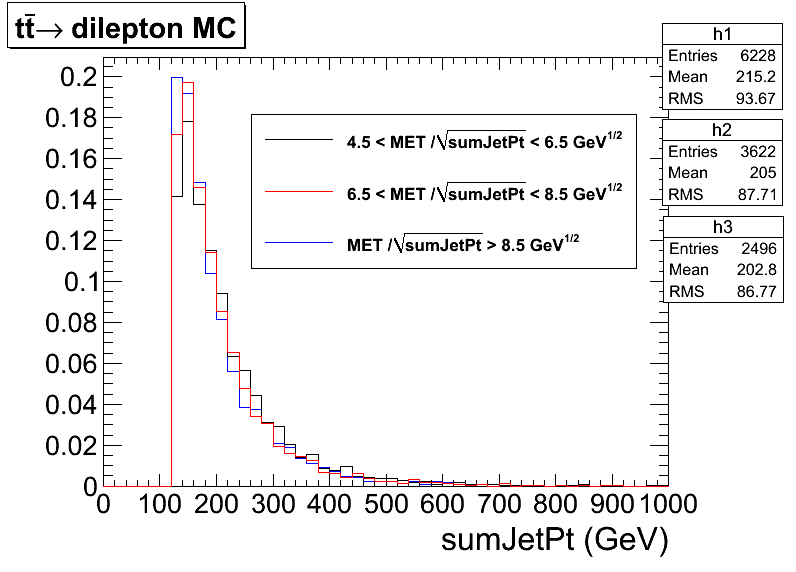
\includegraphics[width=0.48\linewidth]{uncor.png}
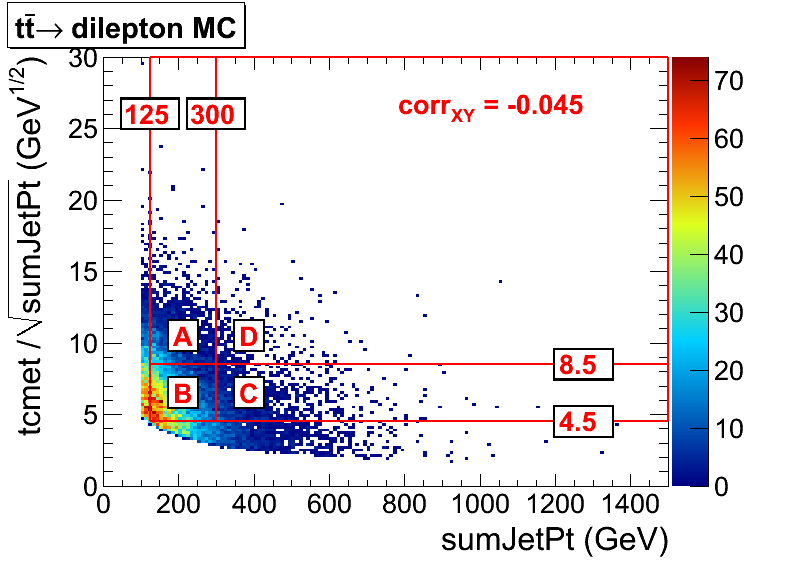
\includegraphics[width=0.48\linewidth]{ttdil_uncor_38X.png}
\caption{\label{fig:uncor}\protect 
Left: distributions of SumJetPt 
in MC $t\bar{t}$ events for different intervals of 
MET$/\sqrt{\rm SumJetPt}$. h1, h2, and h3 refer to the MET$/\sqrt{\rm SumJetPt}$
intervals 4.5-6.5, 6.5-8.5 and $>$8.5, respectively. Right: 
Distributions of MET$/\sqrt{\rm SumJetPt}$ vs. 
SumJetPt for SM Monte Carlo.  Here we also show our choice of ABCD regions. The correlation coefficient
${\rm corr_{XY}}$ is computed for events falling in the ABCD regions.
{\bf THESE PLOTS ARE OLD MC, WILL UPDATE}
}
\end{center}
\end{figure}

We find that in $t\bar{t}$ events \Ht\ and 
$y$ are nearly uncorrelated, 
as demonstrated in Fig.~\ref{fig:uncor} (left).
Thus, we can use an ABCD method in the $y$ vs. \Ht\
plane to estimate the background in a data driven way. We define 4 regions in the 
plane of $y$ vs. \Ht, as shown in Fig.~\ref{fig:uncor} (right).
The region D is the signal region, and the regions A, B and C are control regions.
The predicted background in region D is given by $N_A \times N_C / N_B$.

In Table~\ref{tab:mcabcd}, we quote the \ttbar\ MC expected yields for 1~fb$^{-1}$. In
general we find that the prediction agrees with the observed yield in the signal region within
$\sim$30-50\% for all signal regions. We also study the dependence of the ratio
of observed to predicted signal yields, as a function of the $y$ and \Ht\
requirements used to define the signal region, shown in Fig.~\ref{fig:abcdvar}.
Based on these results, we apply the
scale factors and uncertainties summarized in Table~\ref{tab:cor} to the
predicted background from the ABCD method.


\begin{figure}[hbt]
\begin{center}
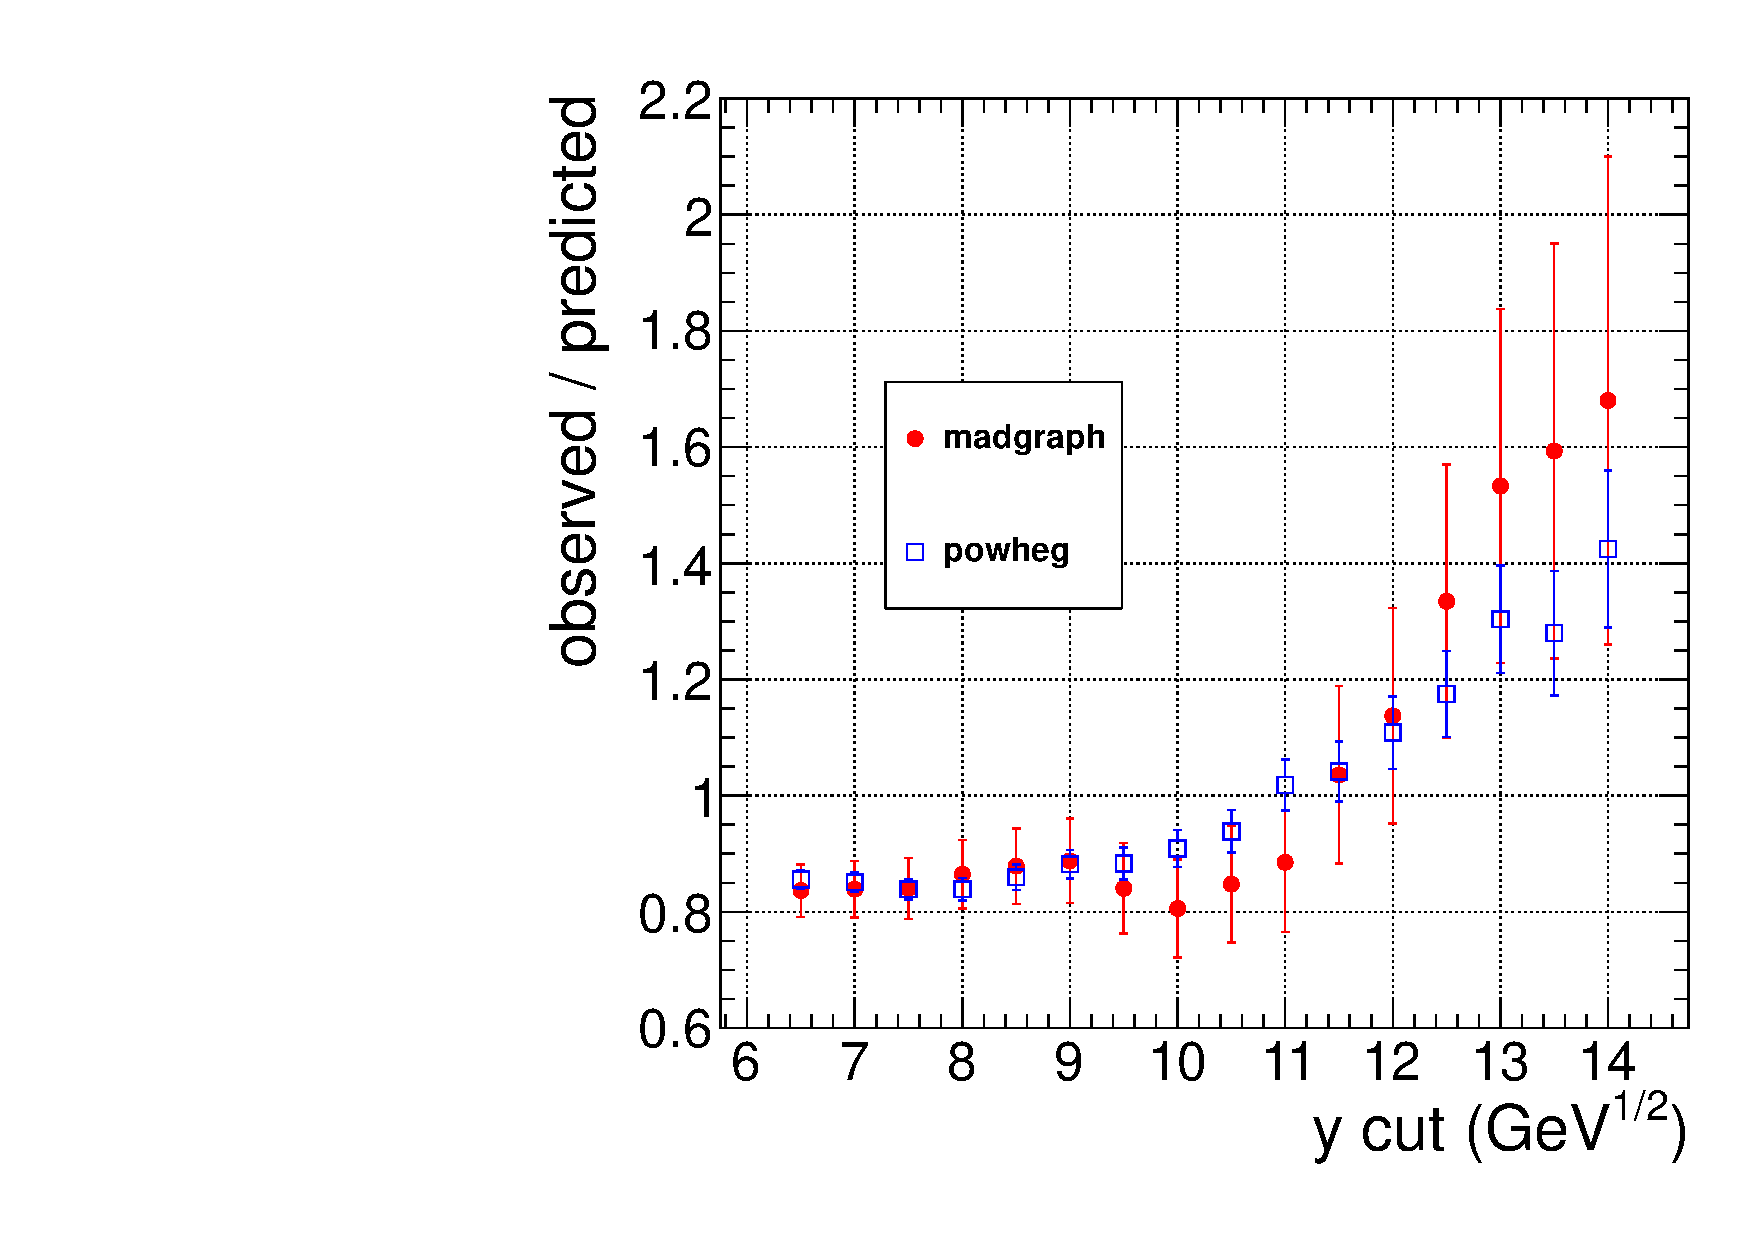
\includegraphics[width=0.48\linewidth]{plots/abcd_y.pdf}
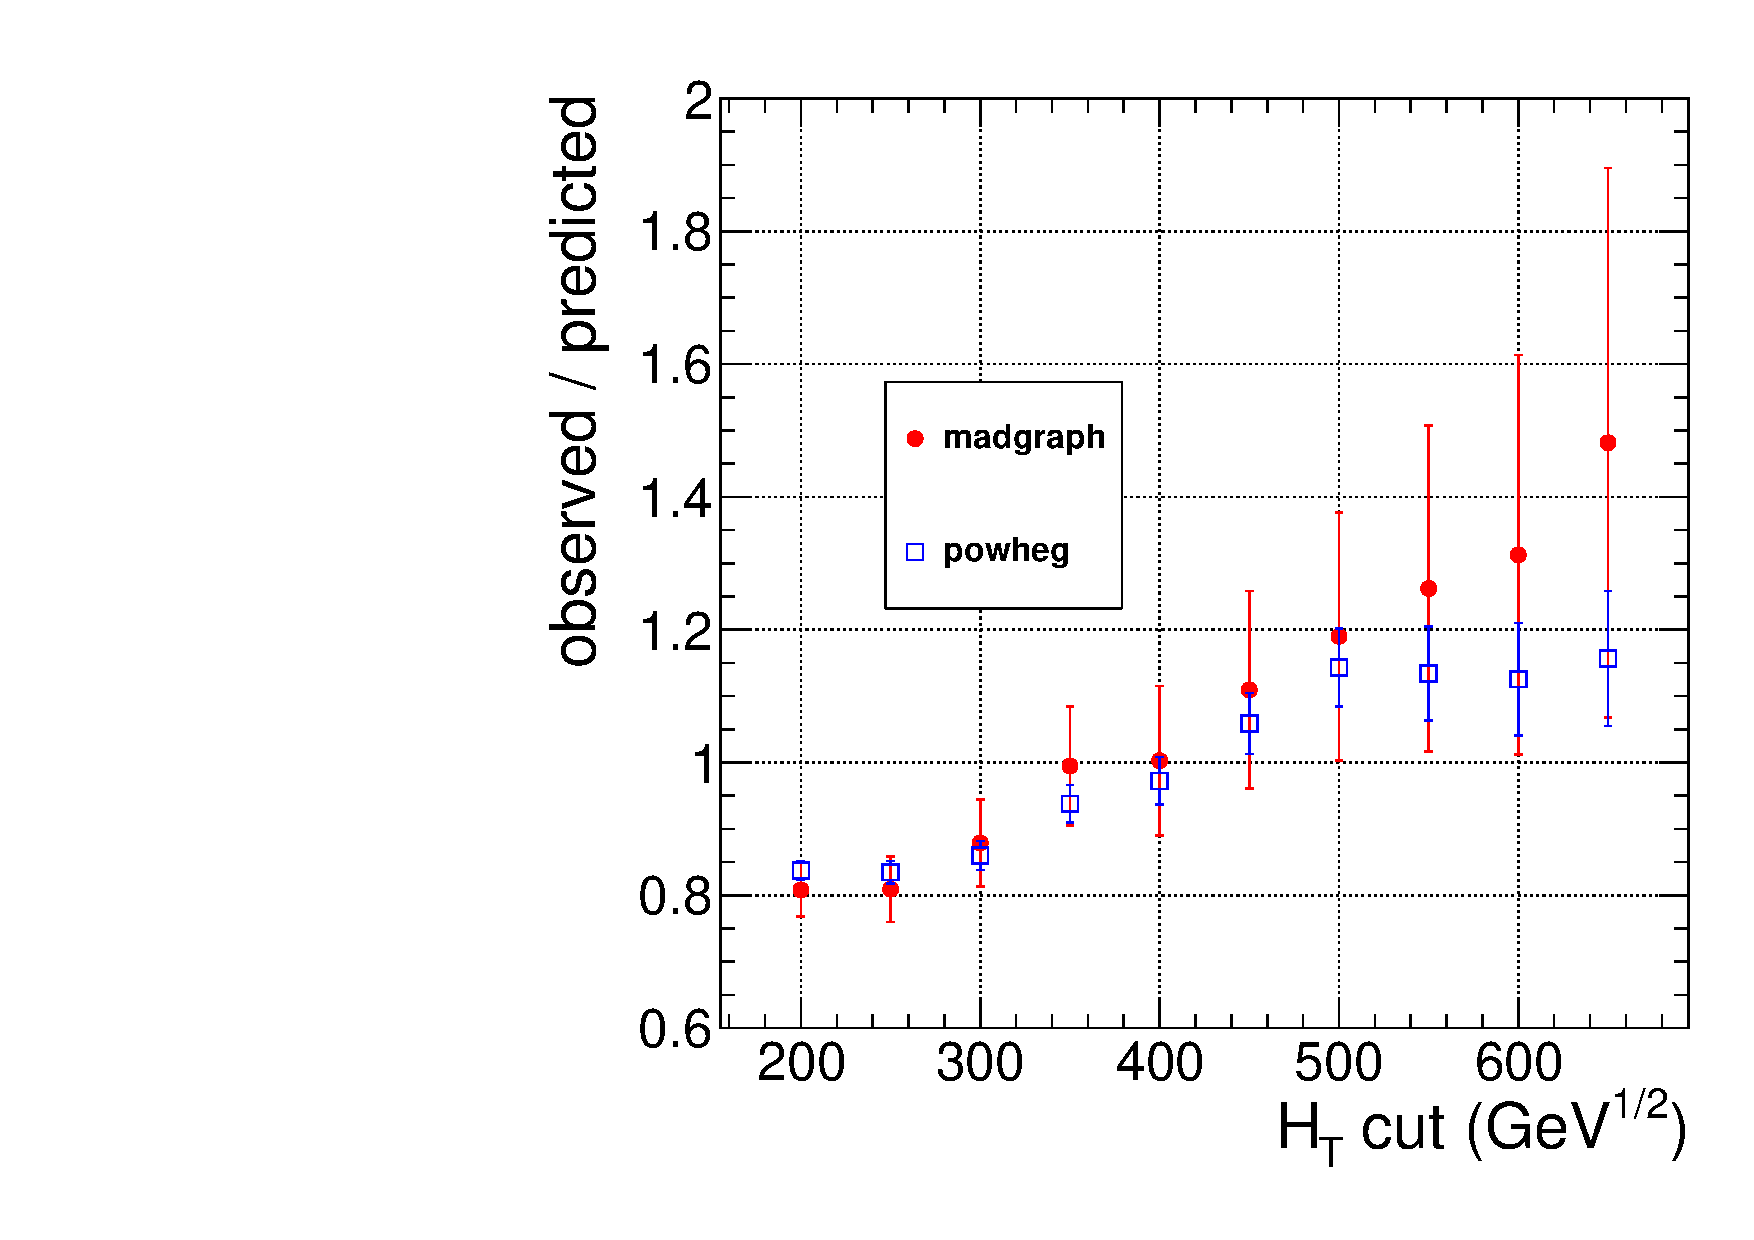
\includegraphics[width=0.48\linewidth]{plots/abcd_ht.pdf}
\caption{\label{fig:abcdvar}\protect Variation of observed/predicted
for the ABCD method as a function of the $y$ and \Ht\ cuts defining
the signal region.}
\end{center}
\end{figure}


\begin{table}[hbt]
\begin{center}
\caption{\label{tab:mcabcd} Expected yields from \ttbar\ MC in 1~fb$^{-1}$ in the four
ABCD regions for the signal regions depicted in Figs.~\ref{fig:abcdData1}-\ref{fig:abcdData3},
as well as the predicted yield in region D given
by A $\times$ C / B and the ratio of the observed signal yield to the prediction. The quoted uncertainties are statistical
only.
}
\begin{tabular}{llccccc|c}
\hline
signal region &           sample  &                A  &                B  &                C  &                D  &   A $\times$ B / C   & obs/pred\\
\hline

\hline

2010 signal region      &   madgraph  & 251.3  $\pm$  6.1  &951.5  $\pm$  11.9  & 165.2  $\pm$  4.9  & 38.3  $\pm$  2.4  & 43.6  $\pm$  1.8  &0.88  $\pm$  0.07 \\
                        &   powheg    & 231.7  $\pm$  2.0  &850.6  $\pm$  3.7   & 157.8  $\pm$  1.6  & 37.0  $\pm$  0.8  & 43.0  $\pm$  0.6  &0.86  $\pm$  0.02 \\

\hline

high $y$ signal region  &   madgraph  & 18.4  $\pm$  1.6   &951.5  $\pm$  11.9  & 165.2  $\pm$  4.9  &  4.9  $\pm$  0.9  &  3.2  $\pm$  0.3  &1.53  $\pm$  0.30 \\
                        &     powheg  & 17.3  $\pm$  0.5   &850.6  $\pm$  3.7   & 157.8  $\pm$  1.6  &  4.2  $\pm$  0.3  &  3.2  $\pm$  0.1  &1.30  $\pm$  0.09 \\

\hline

high \Ht\ signal region &   madgraph  & 251.3  $\pm$  6.1  &951.5  $\pm$  11.9  & 11.1  $\pm$  1.3  &  3.8  $\pm$  0.8  &  2.9  $\pm$  0.3  &1.31  $\pm$  0.30 \\
                        &     powheg  & 231.7  $\pm$  2.0  &850.6  $\pm$  3.7   & 12.5  $\pm$  0.5  &  3.8  $\pm$  0.3  &  3.4  $\pm$  0.1  &1.13  $\pm$  0.08 \\


\hline
%high $y$ signal region  & 

\hline
\end{tabular}
\end{center}
\end{table}


\clearpage

\subsection{Dilepton $P_T$ method}
\label{sec:victory}
This method is based on a suggestion by V. Pavlunin\cite{ref:victory},
and was investigated by our group in 2009\cite{ref:ourvictory} and
in our 2010 analysis~\cite{ref:ospaper}.
The idea is that in dilepton $t\bar{t}$ events the lepton and neutrinos
from $W$ decays have the same $P_T$ spectrum (modulo $W$ polarization 
effects).  One can then use the observed 
$P_T(\ell\ell)$ distribution to model the sum of neutrino $P_T$'s which 
is identified with the \met.

Then, in order to predict the $t\bar{t} \to$ dilepton contribution to a 
selection with \met$+$X, one applies a cut on $P_T(\ell\ell)+$X instead.
In practice one has to rescale the result of the $P_T(\ell\ell)+$X selection
to account for the fact that any dilepton selection must include a 
moderate \met\ cut in order to reduce Drell Yan backgrounds.  This 
is discussed in Section 5.3 of Reference~\cite{ref:ourvictory}; for a \met\
cut of 50 GeV, the rescaling factor is obtained from the MC as

\begin{figure}[hbt]
\begin{center}
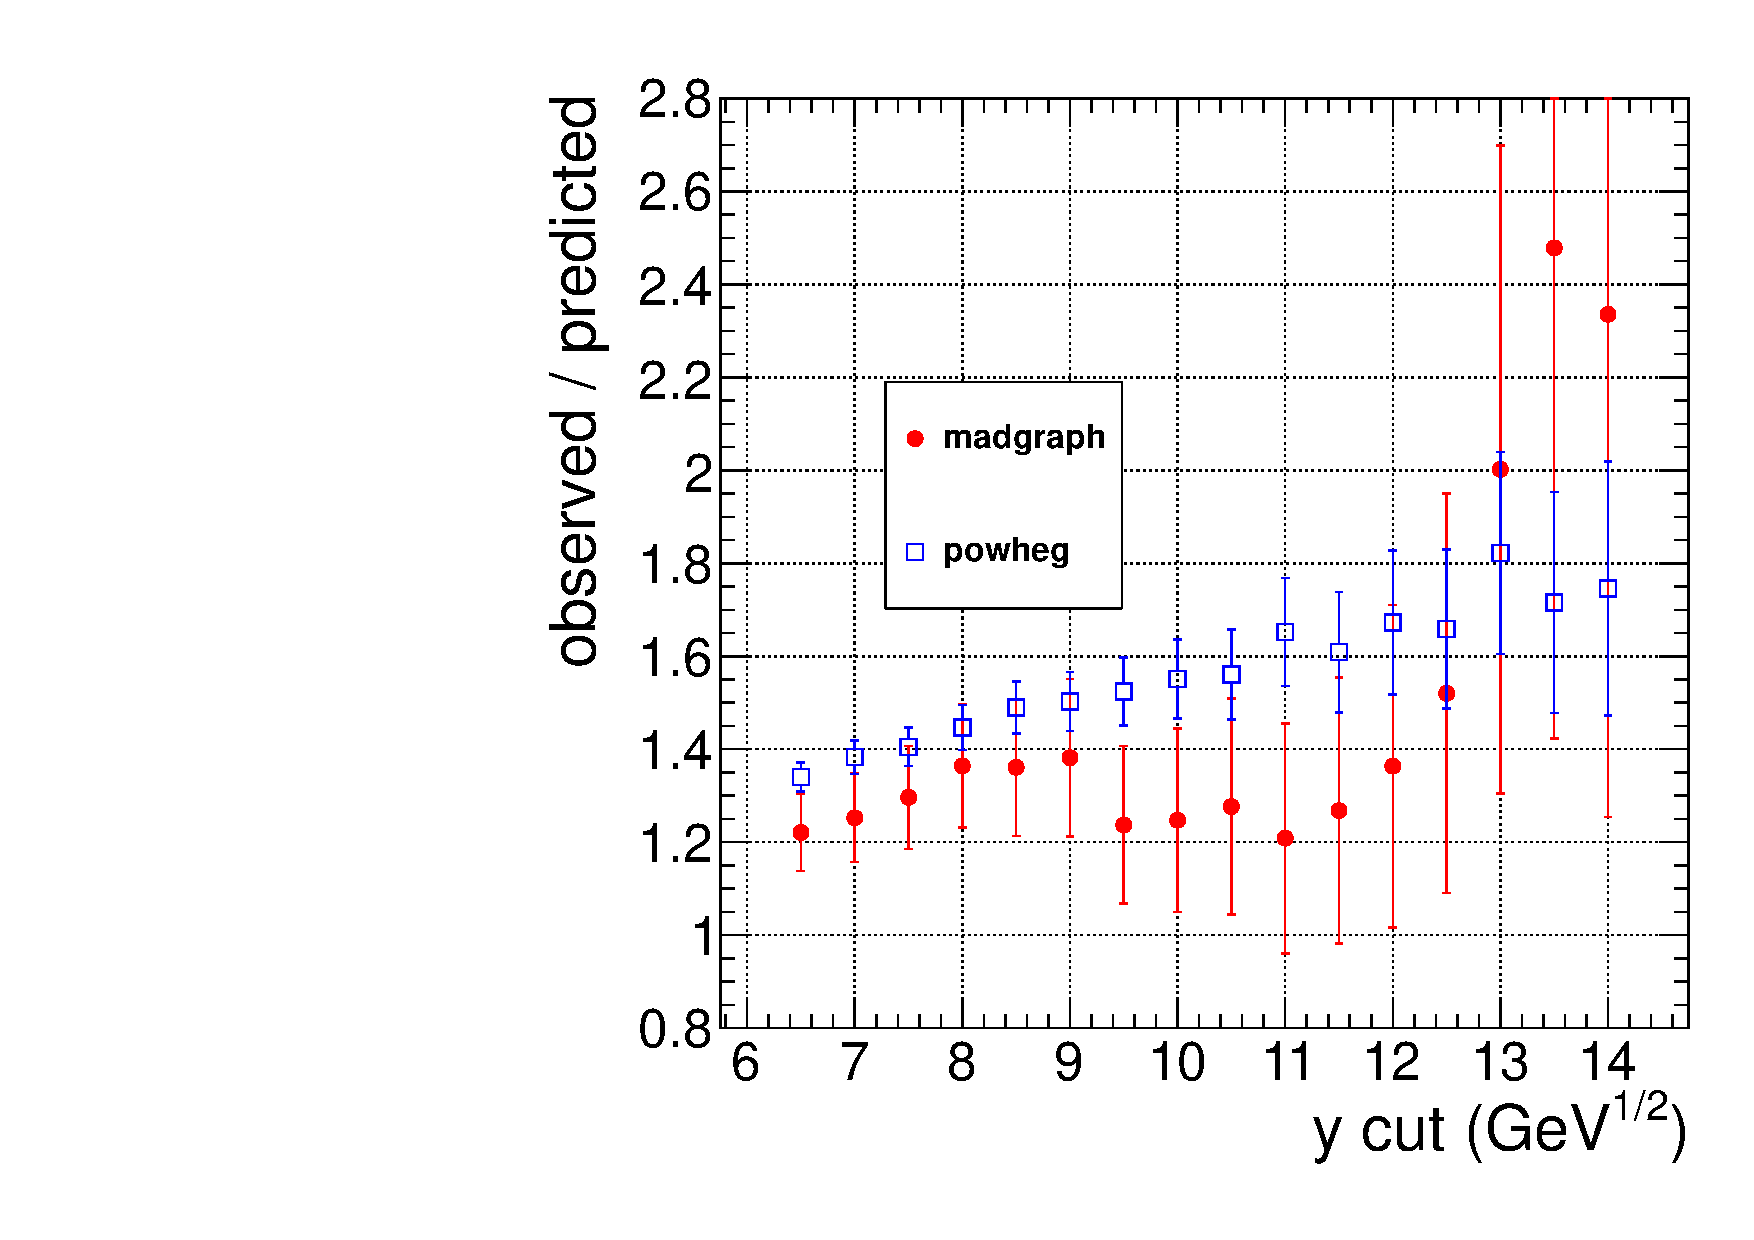
\includegraphics[width=0.48\linewidth]{plots/victory_yvary.pdf}
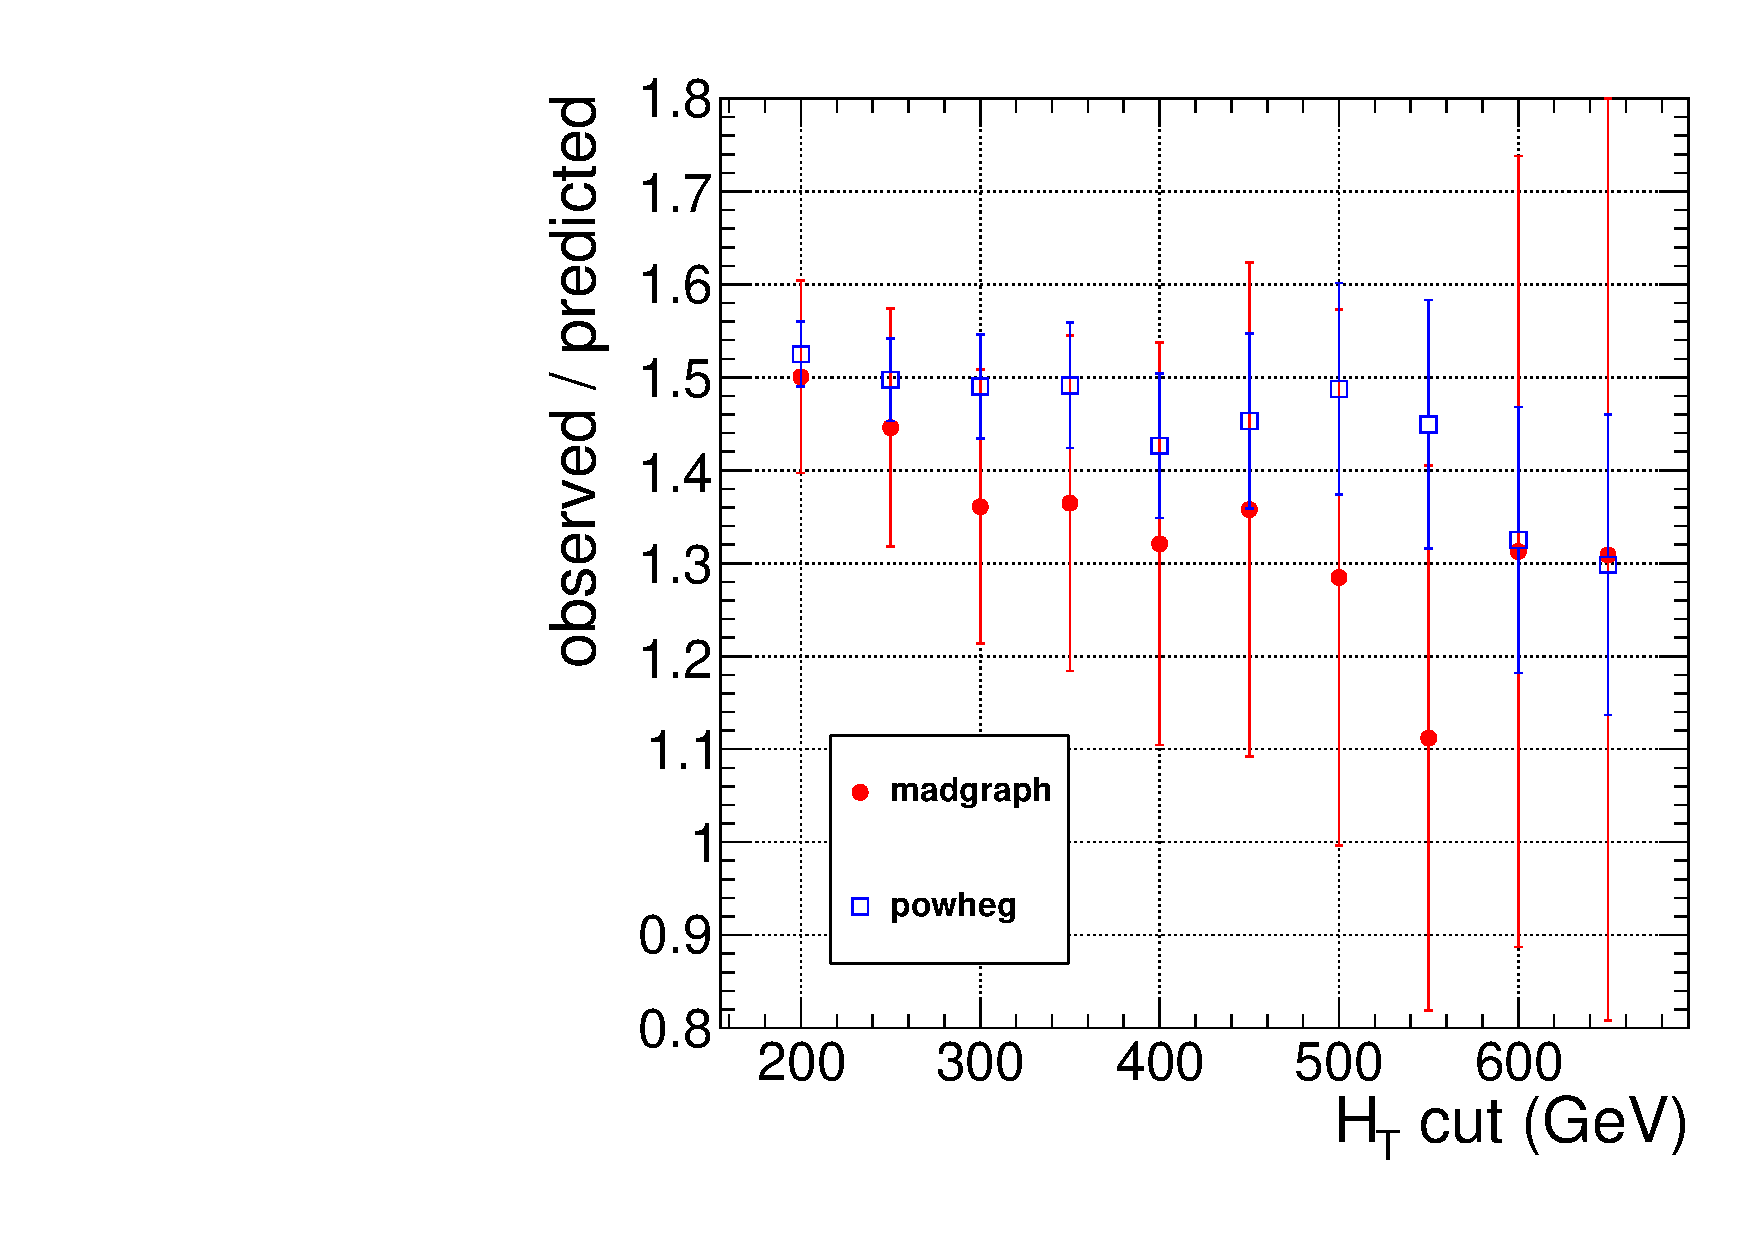
\includegraphics[width=0.48\linewidth]{plots/victory_htvary.pdf}
\caption{\label{fig:victory}\protect Variation of observed/predicted
for the \ptll\ method as a function of the $y$ and \Ht\ cuts defining
the signal region.}
\end{center}
\end{figure}

We summarize the expected results of the \ptll\ method in 1~fb$^{-1}$ \ttbar\ MC in Table~\ref{tab:mcvictory},
and we show the dependence of observed/predicted vs. the signal region requirements in Fig.~\ref{fig:victory}.
Based on these results, we apply the scale factors and uncertainties summarized in Table~\ref{tab:cor} to the
predicted background from the ABCD method. In~\cite{ref:osnote}, we have studied extensively the origin
of the excess of observed vs. predicted events from this method. We found that it is due mostly to 
the $W$ polarization, which results in a harder \pt\ distribution for the $W$ neutrinos than charged leptons.

\begin{table}[hbt]
\begin{center}
\caption{\label{tab:mcvictory} Expected observed and predicted yields in 1~fb$^{-1}$ for \ttbar\ MC for the \ptll\ method, 
and the ratio of the observed signal yield to the prediction. The quoted uncertainties are statistical
only, assuming Gaussian errors.
}
\begin{tabular}{llcc|c}
\hline
signal region &           sample  &                predicted  &                observed  &                obs/pred   \\ 
\hline

\hline

2010 signal region      &   madgraph  & 28.2 $\pm$ 2.5   &      38.3 $\pm$ 2.4   &     1.36 $\pm$ 0.15  \\
                        &   powheg    & 24.8 $\pm$ 0.8   &      37.0 $\pm$ 0.8   &     1.49 $\pm$ 0.06  \\


\hline

high $y$ signal region  &   madgraph  & 2.4 $\pm$ 0.7   &       4.9 $\pm$ 0.9   &     2.00 $\pm$ 0.70  \\
                        &     powheg  & 2.3 $\pm$ 0.2   &       4.2 $\pm$ 0.3   &     1.82 $\pm$ 0.22  \\

\hline

high \Ht\ signal region &   madgraph  & 2.9 $\pm$ 0.8   &       3.8 $\pm$ 0.8   &     1.31 $\pm$ 0.43  \\
                        &     powheg  & 2.9 $\pm$ 0.2   &       3.8 $\pm$ 0.3   &     1.33 $\pm$ 0.14  \\


\hline
%high $y$ signal region  & 

\hline
\end{tabular}
\end{center}
\end{table}

\begin{center}
$ K = \frac{\int_0^{\infty} {\cal N}(\ptll)~~d\ptll~}{\int_{50}^{\infty} {\cal N}(\ptll)~~d\ptll~} = 1.5$
\end{center}

\begin{table}[hbt]
\begin{center}
\caption{\label{tab:cor} Summary of correction factors and systematic uncertainties
for the ABCD and \ptll\ methods in the 3 signal regions.
}
\begin{tabular}{lcc}
\hline
signal region               &           ABCD  &                \ptll  \\
\hline
2010 signal region          &   $1.0 \pm 0.2$ &        $1.4 \pm 0.2$   \\
high $y$  signal region     &   $1.3 \pm 0.3$ &        $1.7 \pm 0.3$   \\
high \Ht\ signal region     &   $1.2 \pm 0.2$ &        $1.3 \pm 0.2$   \\
\hline
\end{tabular}
\end{center}
\end{table}



\subsection{Opposite-Flavor Subtraction}
\label{sec:ofsubtraction}

The opposite-flavor subtraction technique exploits the fact that in \ttbar, the flavor
of the 2 leptons from $W$ decay are uncorrelated. Hence we expect equal rates of same-flavor (SF) 
$ee$ or $\mu\mu$ vs. opposite-flavor (OF) $e\mu$ lepton pairs. In SUSY, the lepton flavors may be 
correlated, producing an excess of SF over OF events. We use the observed 
yield in the OF final state to predict the yields in the SF final state according to:

\begin{center}
$N(ee)     = \frac{1}{2R_{\mu e}}N(e\mu)$ and $N(\mu\mu) = \frac{R_{\mu e}}{2}N(e\mu)$
\end{center}

where $R_{\mu e}$ is the ratio of muon to electron selection efficiencies.
This quantity is evaluated by taking the ratio of the number of observed
$Z \to \mu^+\mu^-$ to $Z \to e^+e^-$ events, in the mass range 76-106 GeV
with no jets or \met\ requirements (see Fig.~\ref{fig:Z}). Alternatively, we can quantify
the excess of SF vs. OF events with the quantity:

\begin{equation}
\label{eq:ofhighpt}
\Delta = R_{\mu e}N(ee) + \frac{1}{R_{\mu e}}N(\mu\mu) - N(e\mu),
\end{equation}

which is predicted to be 0 for processes with uncorrelated lepton flavors. 
For data, we have verified that the contribution from fake leptons in the high lepton \pt\
signal regions is small using the data-driven fake rate method, hence we do not need to 
correct for fake leptons here. In order
for this technique to work, the kinematic selection applied to events in all dilepton
flavor channels must be the same, which is not the case for our default selection because the
$Z$ mass veto is applied only to same-flavor channels. Therefore when applying the OF
subtraction technique we also apply the $Z$ mass veto also to the $e\mu$ channel. 

We will apply this technique to both the high \pt\ dilepton trigger and dilepton-\Ht\ trigger data samples.
In the following, we first apply the technique to \ttbar\ MC with high \pt\ leptons, and then
to \ttbar\ MC with low \pt\ leptons.

\subsubsection{OF subtraction: Application to high \pt\ lepton sample}

We begin by applying the OF subtraction technique to \ttbar\ MC with leptons passing \pt\ $>$ (20,10) GeV.
Here we extract $R_{e\mu}$ by taking the ratio of $Z \to \mu^+\mu^-$ vs. $Z \to e^+e^-$ events in the
window 76--106 GeV in DY MC. The results are summarized in Table~\ref{tab:mcof}, where we find
values of $\Delta$ consistent with 0, as expected.

\begin{table}[hbt]
\begin{center}
\caption{\label{tab:mcof} Expected yields in 1~fb$^{-1}$ \ttbar\ MC for the OF subtraction method,
and the quantity $\Delta$, defined in Eq.~\ref{eq:ofhighpt}.
The quoted systematic uncertainty refers to that of $R_{\mu e}$.
}
\begin{tabular}{llccc|c}
\hline
region                  &     sample  &       $N(ee)$     &      $N(\mu\mu)$   &     $N(e\mu)$      &         $\Delta$   \\ 
\hline

\hline

preselection region     &   madgraph  & 431.1 $\pm$ 8.0   &  531.3 $\pm$ 8.9   &  945.8 $\pm$ 11.8  &  11.8 $\pm$ 16.8 (stat) $\pm$ 1.1 (syst)   \\
                        &   powheg    & 383.1 $\pm$ 2.5   &  492.9 $\pm$ 2.9   &  876.2 $\pm$ 3.8   &  -7.0 $\pm$  5.4 (stat) $\pm$ 0.8 (syst)   \\

\hline

2010 signal region      &   madgraph  &   7.4 $\pm$ 1.0   &   10.7 $\pm$ 1.3   &   14.5 $\pm$ 1.5   &   3.3 $\pm$  2.2 (stat) $\pm$  0.04 (syst) \\
                        &   powheg    &   7.2 $\pm$ 0.3   &    8.6 $\pm$ 0.4   &   16.8 $\pm$ 0.5   &  -1.1 $\pm$  0.7 (stat) $\pm$  0.03 (syst) \\

\hline
%high $y$ signal region  & 

\hline
\end{tabular}
\end{center}
\end{table}

\subsubsection{OF subtraction: Application to low \pt\ lepton sample}
\label{sec:oflowpt}

In this section, we apply the OF subtraction technique to \ttbar\ MC with
leptons passing \pt\ $>$ (10,5) GeV but not passing \pt\ $>$ (20,10) GeV
(in order to remove overlap with the high lepton \pt\ sample).
The OF subtraction in the low lepton \pt\ regime is complicated by 2 factors:

\begin{itemize}
\item The ratio of muon to electron selection efficiencies $R_{\mu e}$ increases significantly 
at low \pt, due to a drop in the electron selection efficiency.
\item We reconstruct muons down to \pt\ $>$ 5 GeV but electrons only to \pt\ $>$ 10 GeV.
\end{itemize}

Our strategy is the following:

\begin{itemize}
\item Evaluate $R_{\mu e}$ from \ttbar\ MC. 
\item Parameterize $R_{\mu e}$ as a function of lepton \pt. For now we split in 2 bins, $10 < $ \pt\ $ < 20$ GeV
and \pt\ $>$ 20 GeV.
\item For data, we will apply to $R_{\mu e}$ a trigger efficiency correction and subtract the 
expected contribution from fake leptons from the data-driven fake rate method (but neither correction is performed for the
MC studies in this section).
\item We first apply the OF subtraction to the preselection region, and then to the signal region. 
\end{itemize}

\begin{figure}[tbh]
\begin{center}
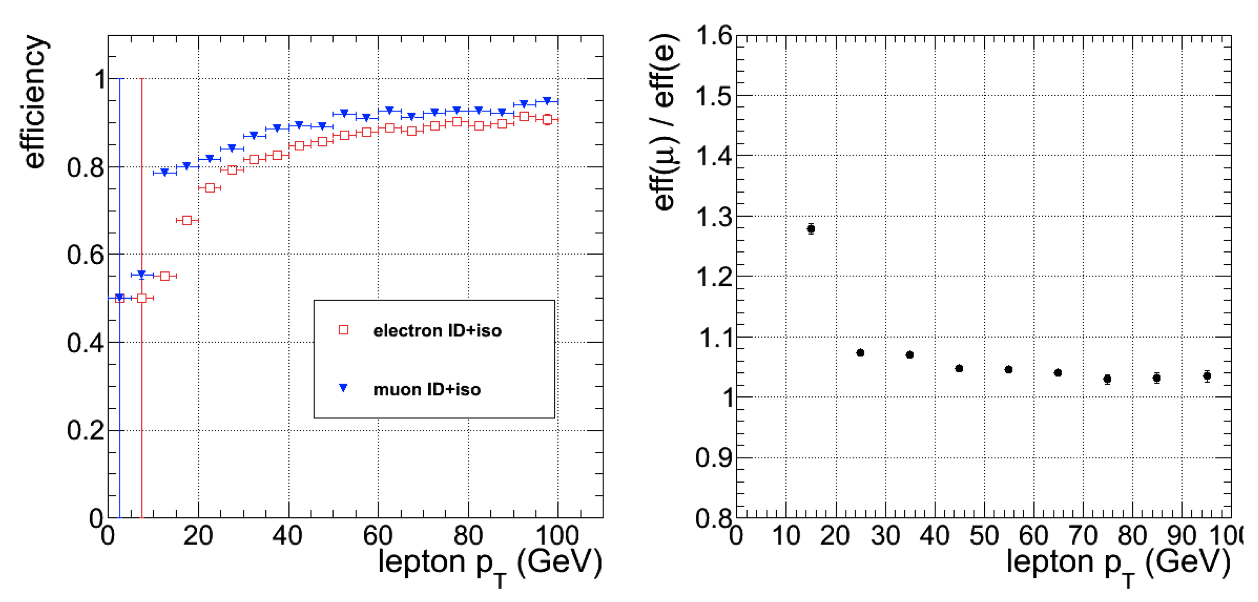
\includegraphics[width=1\linewidth]{plots/r_ttmadgraph.png}
\caption{\label{fig:rtt}\protect 
Left: the electron and muon selection efficiencies, as a function of lepton \pt, extracted
from \ttbar\ MC. Right: the ratio $R_{\mu e}$ of muon to electron selection efficiencies
as a function of lepton \pt.
}
\end{center}
\end{figure}

We begin by examining the dependence of $R_{\mu e}$ on lepton \pt, as shown in Fig.~\ref{fig:rtt}.
We find that $R_{\mu e}$ increases in the region \pt\ 10--20 GeV, but is roughly constant for \pt\ $>$ 20 GeV.
Hence we take $R_{\mu e}^{10-20} = 1.28$ for \pt\ 10--20 GeV and $R_{\mu e}^{>20} = 1.08$ for \pt\ $>$ 20 GeV, and assign
a 5\% systematic uncertainty.

Next, to take into account the fact the electrons and muons have a different \pt\ range, we split the low \pt\
sample into events with leptons passing \pt\ $>$ (10,10) GeV, denoted in the following as (10,10), and 
events with leptons passing \pt\ $>$ (10,5) GeV but not passing \pt\ $>$ (10,10) GeV, denoted in the following
as (10,5). We find the following relations, expected for backgrounds with uncorrelated lepton flavors:

\begin{itemize}
\item $N(ee)(10,10)     = 1/(2 R_{\mu e}^{10-20}) N(e\mu)(10,10)$
\item $N(\mu\mu)(10,10) = (R_{\mu e}^{10-20}/2) N(e\mu)(10,10)$
\item $N(\mu\mu)(10,5)  = R_{\mu e}^{>20} N(e\mu)(10,5)$
\end{itemize}

Note that for (10,10) events, both leptons are in the range \pt\ 10--20 GeV, hence the relevant efficiency
ratio is $R_{\mu e}^{10-20}$. For (10,5) events, both $ee$ and $\mu\mu$ events have a muon with \pt\ 5--10 GeV
and an additional lepton with \pt\ $>$ 10 GeV. In most cases the leading lepton has \pt\ $>$ 20 GeV,
hence we use $R_{\mu e}^{>20}$ for these events.
{\bf TECHNICALLY, ONE SHOULD SPLIT (10,5) EVENTS DEPENDING ON LEADING LEPTON PT 10-20 vs. $>$20, AND USE CORRESPONDING R VALUE.}
 
In this case we find the following expression for $\Delta$, quantifying the excess of SF vs. OF yields:

\begin{equation}
\label{eq:oflowpt}
\Delta = R_{\mu e}^{10-20} N(ee)(10,10) + 1/R_{\mu e}^{10-20} N(\mu\mu)(10,10) + 1/R_{\mu e}^{>20} N(\mu\mu)(10,5) - N(e\mu)(10,10) - N(e\mu)(10,5)
\end{equation}

In Table~\ref{tab:mcoflowpt} we apply this technique to \ttbar\ MC. As expected, we find $\Delta$ consistent with 0.
 

\begin{table}[hbt]
\begin{center}
\footnotesize
\caption{\label{tab:mcoflowpt} Expected yields in 1~fb$^{-1}$ \ttbar\ MC for the OF subtraction method in the low lepton \pt\ regime,
and the quantity $\Delta$, defined in Eq.~\ref{eq:oflowpt}. The quoted systematic uncertainty refers to that of $R_{\mu e}$.
}
\begin{tabular}{llccccc|c}
\hline
region                  &     sample  & $N(ee)(10,10)$ & $N(\mu\mu)(10,10)$ & $N(e\mu)(10,10)$ & $N(\mu\mu)(10,5)$ & $N(e\mu)(10,5)$ & $\Delta$  \\ 
\hline

\hline

preselection region     &   madgraph  & 3.4 $\pm$ 0.7  & 4.9 $\pm$ 0.9      & 6.4 $\pm$ 1.0    & 22.9 $\pm$ 1.8    & 18.2 $\pm$ 1.6 &  4.8 $\pm$ 2.8 (stat) $\pm$ 1.0 (syst) \\  
                        &   powheg    & 2.5 $\pm$ 0.2  & 4.4 $\pm$ 0.3      & 7.0 $\pm$ 0.3    & 19.0 $\pm$ 0.6    & 16.6 $\pm$ 0.5 &  0.6 $\pm$ 0.9 (stat) $\pm$ 0.9 (syst) \\

\hline
2010 signal region      &   madgraph  & 0.0 $\pm$ 0.0  & 0.4 $\pm$ 0.3      & 0.6 $\pm$ 0.3    & 1.0 $\pm$ 0.4     & 0.7 $\pm$ 0.3  & -0.0 $\pm$ 0.6 (stat) $\pm$ 0.1 (syst) \\
                        &   powheg    & 0.1 $\pm$ 0.0  & 0.2 $\pm$ 0.1      & 0.4 $\pm$ 0.1    & 1.4 $\pm$ 0.2     & 1.1 $\pm$ 0.1  &  0.1 $\pm$ 0.2 (stat) $\pm$ 0.1 (syst) \\

\hline
\end{tabular}
\end{center}
\end{table}



